\section{figuras}

\begin{figure}[htbp] %htbp = insere onde der ou use H = para inserir obrigatoriamente onde deseja (Este ultimo se importar o pacote FLOAT)
	\centering
	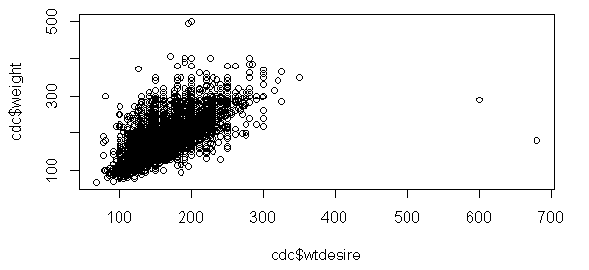
\includegraphics[width=0.8\textwidth]{figuras/q1.PNG}
	\caption{Figura-Q1}
	\label{Nome-da-legenda-da-figura1}
\end{figure}

\begin{figure}[htbp] %htbp = insere onde der ou use H = para inserir obrigatoriamente onde deseja (Este ultimo se importar o pacote FLOAT)
	\centering
	\includegraphics[width=0.8\textwidth]{figuras/q2.PNG}
	\caption{Figura-Q2}
	\label{Nome-da-legenda-da-figura2}
\end{figure}